\begin{surferPage}[Barth-flaten]{Barths flate av sjette grad}
Denne flaten av sjette grad ble konstruert av Wolf Barth i 1996.
    
    Barths flate har til sammen $65$ singulariteter. 
    En flate av sjette grad kan ikke ha flere, noe som Jaffe og Ruberman viste kort tid etter at Barth konstruerte denne flaten. Barths verdensrekord er derfor uslåelig!


Barths konstruksjon var en stor overraskelse fordi man lenge hadde trodd at flater av sjette grad bare kunne ha $64$ singulariteter.

En påfallende egenskap ved flaten, er at den har symmetrien til et ikosaeder, som er en flate bestående av 20 likesidede trekanter. Figuren viser et ikosaeder og dets symmetriplan:    
    % 
  \begin{center}
      \vspace*{-0.1cm}
      \begin{tabular}{@{}c@{\ \ }c@{\,}c@{}}
        \begin{tabular}{@{}c}
          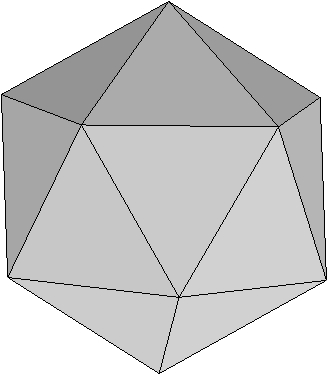
\includegraphics[width=1.4cm]{./../../common/images/icosah}
        \end{tabular}
        &
        \begin{tabular}{@{}c}
          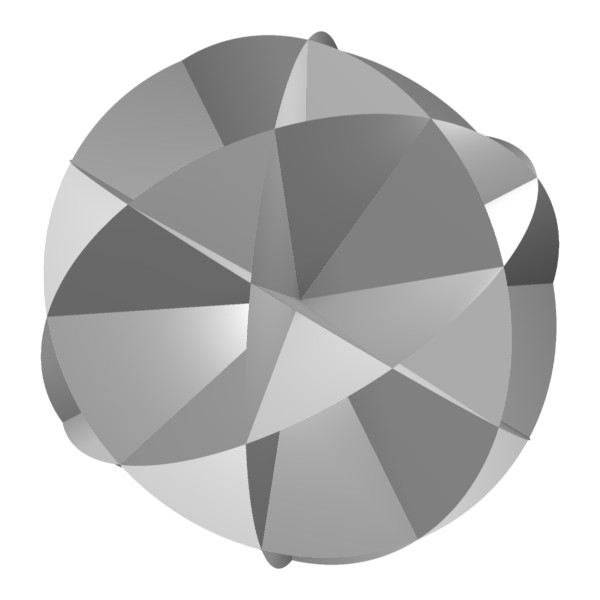
\includegraphics[width=1.4cm]{./../../common/images/barth_sextic_planes}
        \end{tabular}
        &
        \begin{tabular}{c@{}}
          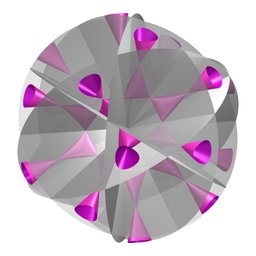
\includegraphics[width=1.4cm]{./../../common/images/barth_sextic_and_planes}
        \end{tabular}
      \end{tabular}
    \end{center}
    \vspace*{-0.1cm}

   Barths flate av sjette grad tilfredsstiller ligningen  
    $P_6 - \alpha K^2=0,$ hvor $P_6$
    er de seks symmetriplanene, $K=x^2+y^2+z^2-1$ er enhetskula (kule med radius 1) og  
    $\alpha=\frac{1}{4}(2+\sqrt{5})$.
\end{surferPage}
